%%%%%%%%%%%%%%%%%%%%%%%%%%%%%%%%%%%%%%%%%%%%%%%%%%%%%%%%%%%
\section{Theory}
\label{sec:theory}
%%%%%%%%%%%%%%%%%%%%%%%%%%%%%%%%%%%%%%%%%%%%%%%%%%%%%%%%%%%
\begin{figure*}[!htb]
\begin{center}
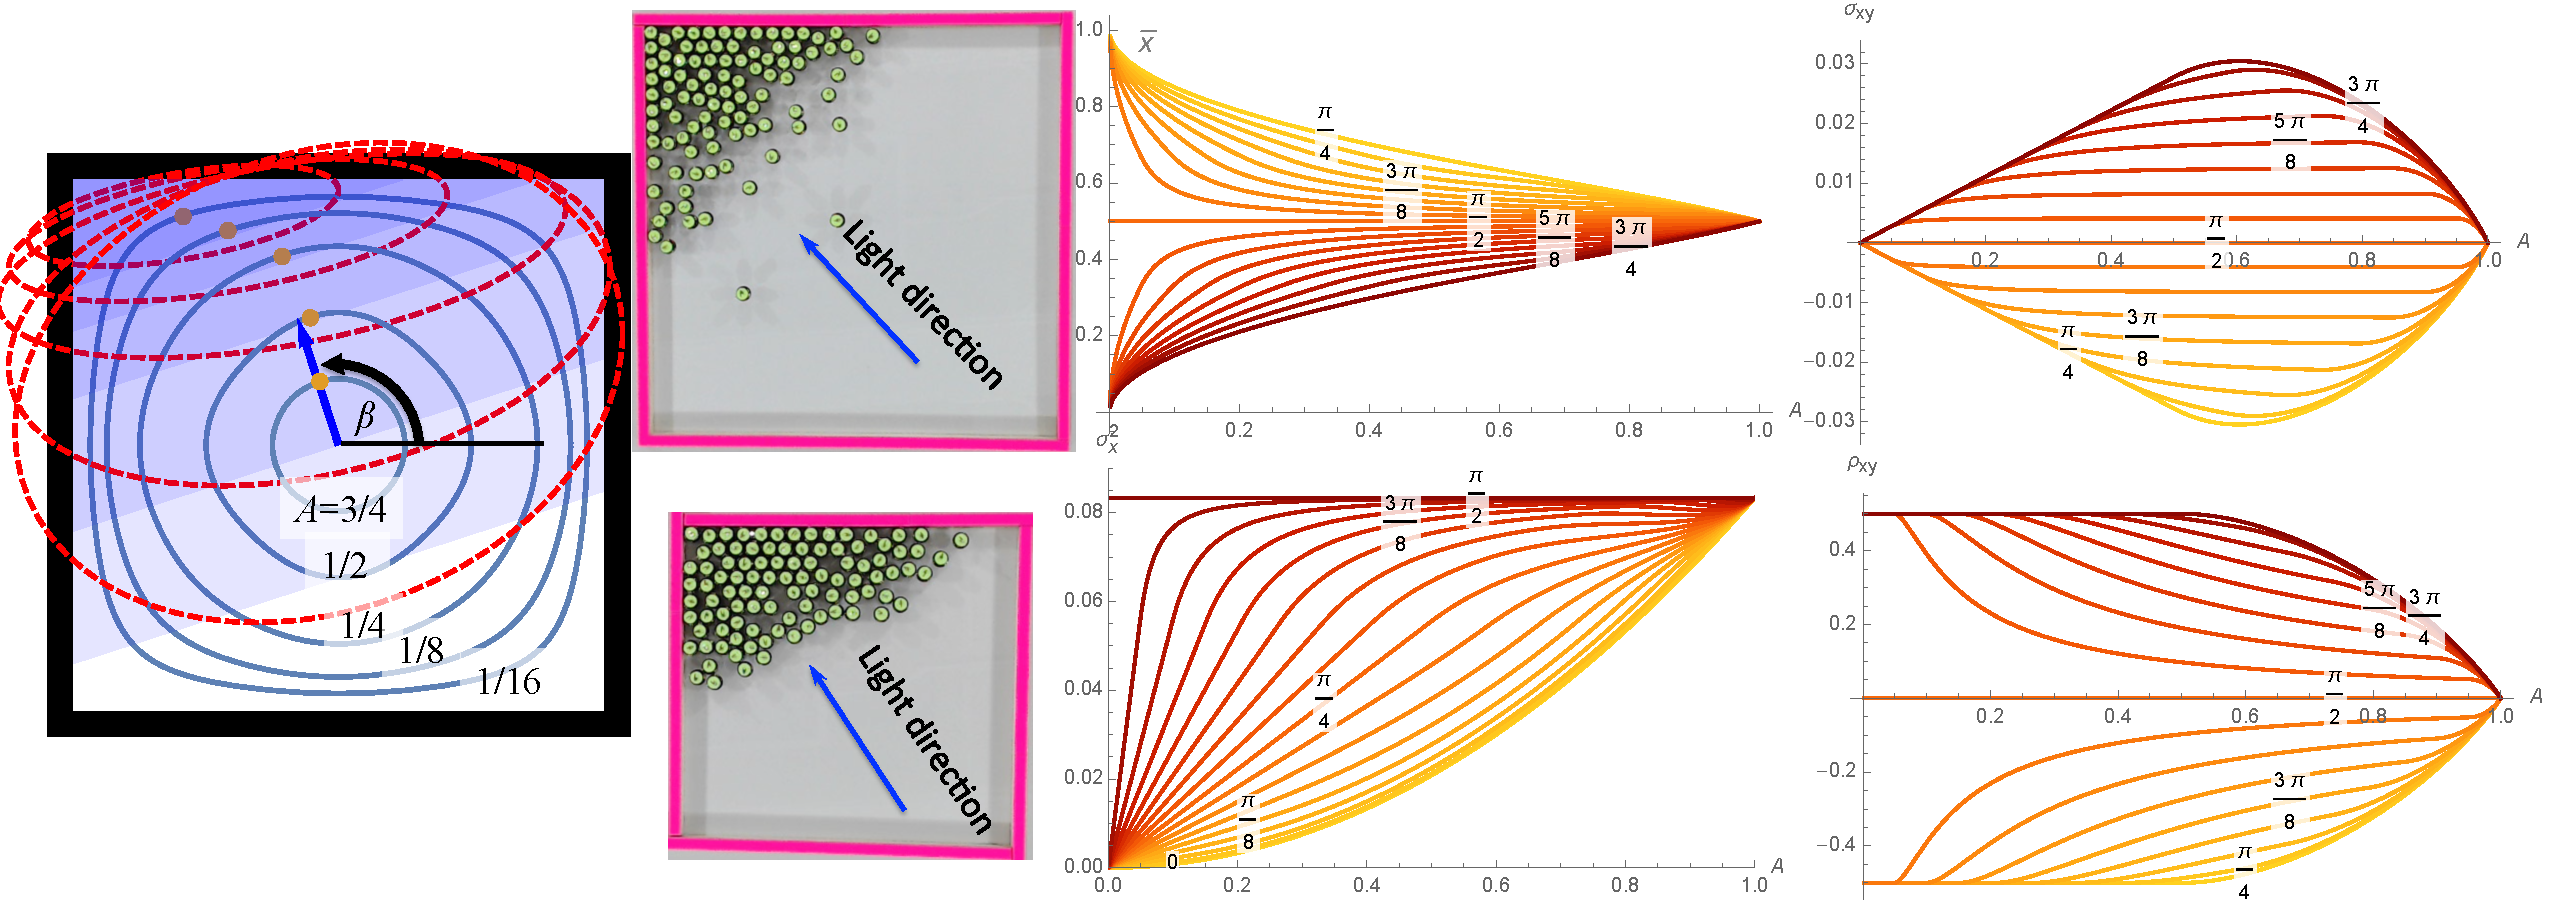
\includegraphics[width=\linewidth]{SquareFill.pdf} 
\caption{Pushing the swarm against a square boundary wall allows limited control of the shape of the swarm, as a function of swarm area $A$ and the commanded movement direction $\beta$. Left plot shows locus of possible mean positions for five values of $A$.  The locus morphs from a square to a circle as $A$ increases.  The covariance ellipse for each $A$ is shown with a dashed line. Center shows two corresponding arrangements of kilobots.  At right is $\bar{x}(A), \sigma_{xy}(A), \sigma_x^2(A),$ and $\rho(A)$ for a range of $\beta values$. See online interactive demonstration at [withheld for double-blind review].}
\label{fig:CircleFill}
\end{center}
\end{figure*} 
\begin{figure*}[!htb]
\begin{center}
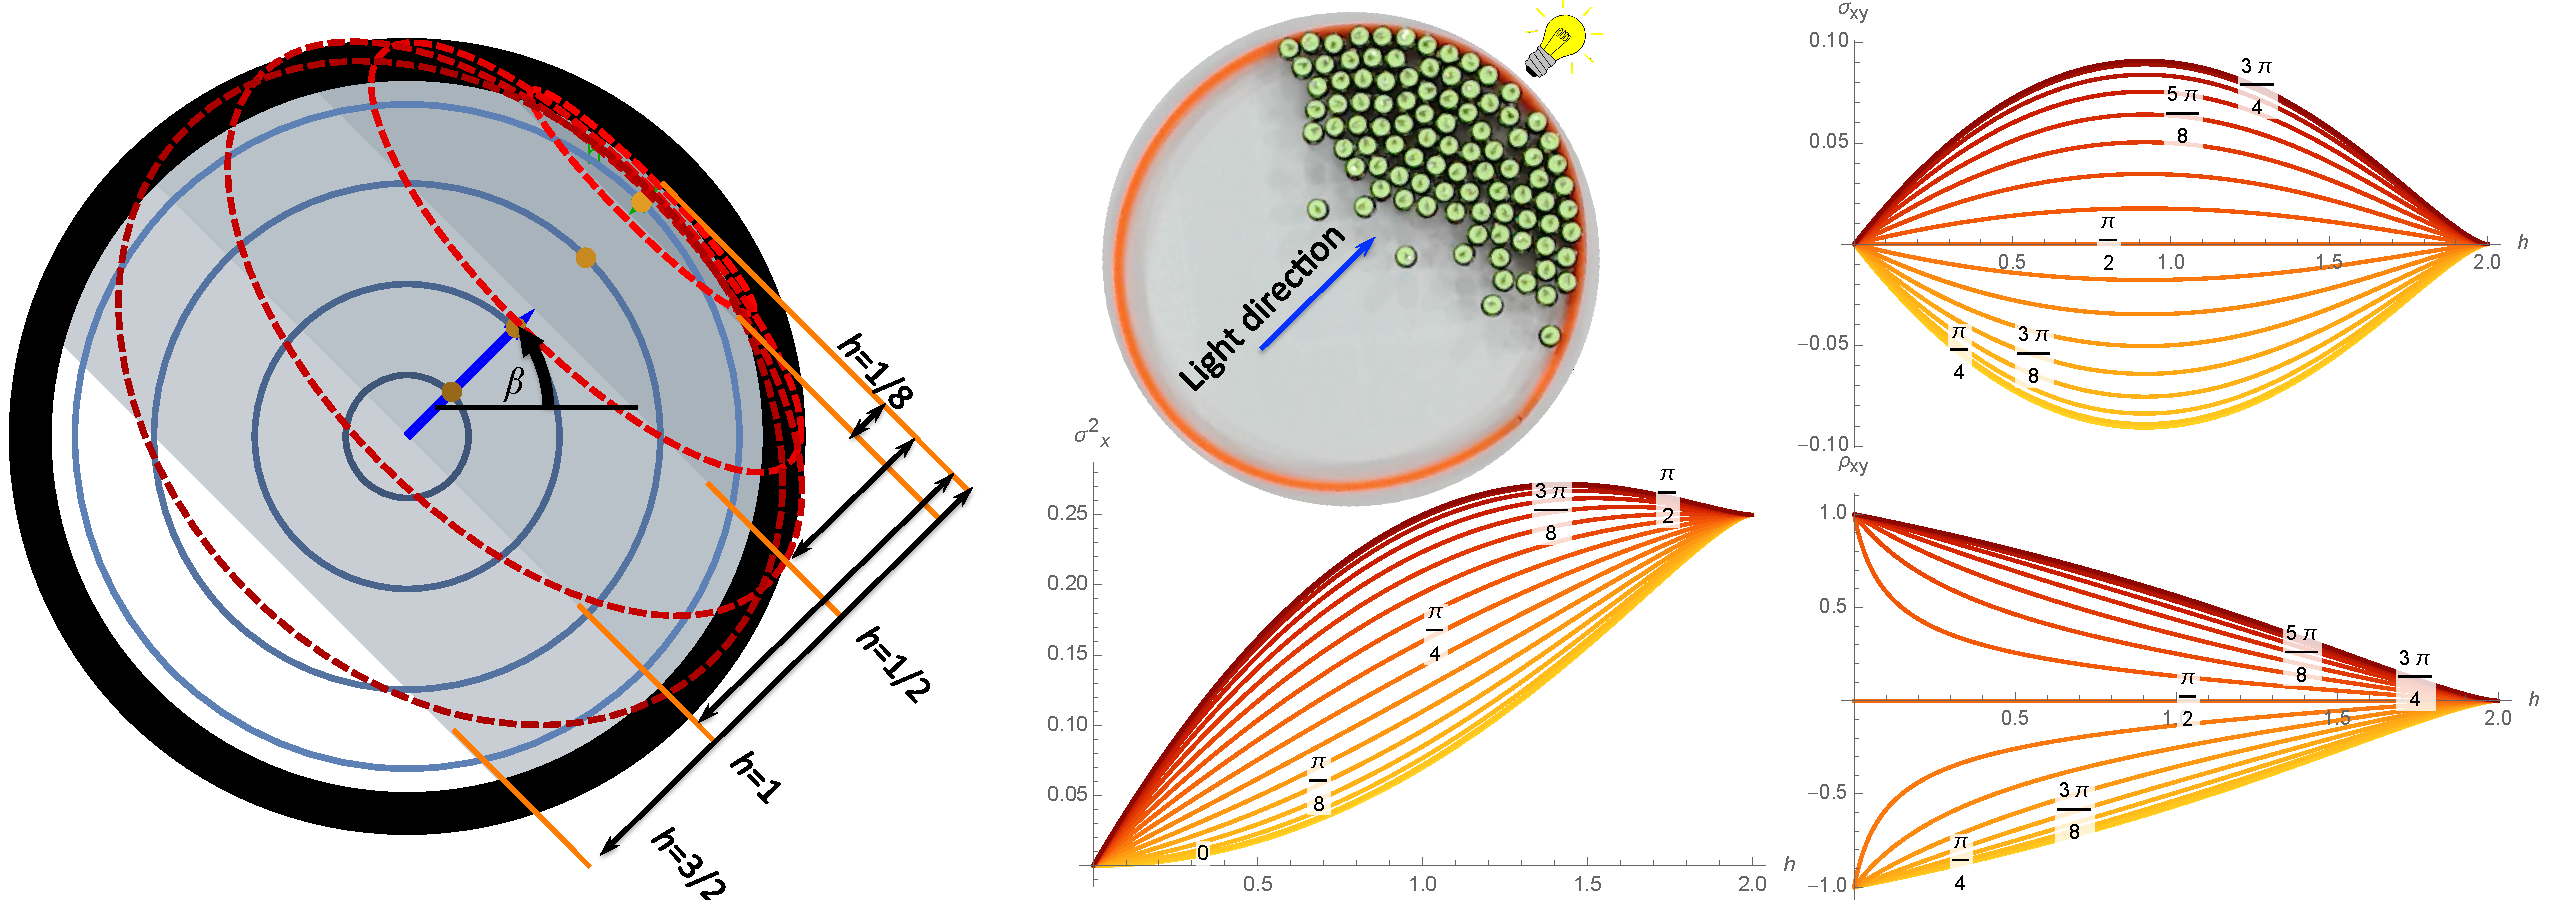
\includegraphics[width=\linewidth]{CircleFill.pdf} 
\caption{Pushing the swarm against a circular boundary wall allows limited control of the shape of the swarm, as a function of the fill level $h$ and the commanded movement direction $\beta$. Left plot shows locus of possible mean positions for four values of $h$. The locus of possible mean positions are concentric circles. See online interactive demonstration at [withheld for double-blind review].}
\label{fig:CircleFill}
\end{center}
\end{figure*} 

\subsection{Controlling Covariance: Fluid Settling In a Tank}\label{subsec:FluidInTank}
One method to control a swarm's shape in a bounded workspace is to simply push in a given direction until the swarm conforms to the boundary.
\paragraph{Square workplace}
This section examines the mean, variance,  covariance and correlation of a very large swarm of robots as they move inside a square workplace under the influence of gravity pointing in the direction $\beta$. The swarm is large, but the robots are small in comparison, and together cover an area of constant volume $A$. Under a global input such as gravity, they flow like water, moving to a side of the workplace and forming a polygonal shape. 

The range of possible angles for the global input angle $\beta $ is [0,2$\pi $). In this range of angles, the swarm assumes eight different polygonal shapes. The shapes alternate between triangles and trapezoids when the area $A$$<$1/2, and alternate between squares with one corner removed and trapezoids when $A$$>$1/2.

Computing the means, variances, covariance, and correlation requires integrating over the area containing the swarm.  One way is to use an indicator function $\bm{1}_A(x,y)$ that returns 1 if inside the region containing the swarm, and 0 else. The formulas for means $(\bar{x},\bar{y})$, covariance $(\sigma^2_x,\sigma^2_y,\sigma_{xy})$, and correlation $\rho_{xy}$ are as follows, integrated over the unit square with $x$ and $y$ from 0 to 1:

\begin{equation}\label{eq:meanInSquareWorkspace}
\bar{x} =\frac{\iint x \bm{1}_A(x,y)dxdy}{A}
\text{, }
\bar{y}=\frac{\iint y \bm{1}_A(x,y)dxdy}{A}
\end{equation}

\begin{align}\label{eq:varInSquareWorkspace}
\sigma^2_x &=\frac{\iint \left(x-\bar{x}\right)^2 \bm{1}_A(x,y) dx dy}{A}, \\
\sigma^2_y &=\frac{\iint  \left(y-\bar{y}\right)^2 \bm{1}_A(x,y) dx dy}{A}
\end{align}

\begin{align}\label{eq:covAndcorrInSquareWorkspace}
\sigma_{xy} &= \frac{\iint  \left(x-\bar{x}_x\right) \left(y-\bar{y}\right) \bm{1}_A(x,y) dx dy}{A},\\
\rho_{xy} &= \frac{\sigma^2_x}{\sigma_x\sigma_y}
\end{align}

Rather than using an indicator function, the region of integration can be changed to only include the polygon containing the swarm. If the force angle is $\beta$, the mean when the swarm is in the lower-left corner is:
\begin{align}\label{eq:meanInSquareWorkspaceLL}
\bar{x}(A,\beta) &= \frac{\int_0^{\sqrt{2} \sqrt{-A \tan (\beta )}} \left(\int_0^{\sqrt{2} \sqrt{-A \cot (\beta )}+x \cot (\beta )} x \, dy\right) \, dx}{A} \nonumber \\
	&=\frac{1}{3} \sqrt{2} \sqrt{A \tan (\beta )}\\
\bar{y}(A,\beta) &= \frac{\int_0^{\sqrt{2} \sqrt{-A \tan (\beta )}} \left(\int_0^{\sqrt{2} \sqrt{-A \cot (\beta )}+x \cot (\beta )} y \, dy\right) \, dx}{A} \nonumber\\
	&=\frac{1}{3} \sqrt{2} \sqrt{A \cot (\beta )}
\end{align}
The full equations are included in the appendix, and are summarized in Fig.~\ref{fig:CircleFill}. A few highlights are that the correlation is maximized when the swarm is in a triangular shape, and is $\pm$1/2. The covariance of a triangle is always $\pm(A/18)$. Variance is minimized in the direction of $\beta$ and minimized orthogonal to $\beta$ when the swarm is in a rectangular shape. The range of mean positions are maximized when $A$ is small.

\paragraph{Circular workplace}
Though rectangular boundaries are common in artificial workspaces, biological workspaces are usually rounded.
Similar calculations can be computed for a circular workspace.  
For notational simplicity, the swarm will be parameterized by the global control input signal $\beta$ and the fill-level $h$, and the workspace is a circle centered at (0,0) with radius 1 and thus area $\pi$.
Under a global input, the robot swarm fills the region under a chord with area
\begin{align}
A(h) = \cos^{-1}(1-h)-(1-h) \sqrt{(2-h) h}
\end{align}
For a circular workspace, the locus of mean positions are aligned with $\beta$ and the mean position is at radius $r(h)$ from the center:
\begin{align}
r(h) = \frac{2 (-(h-2) h)^{3/2}}{3 \left(\sqrt{-(h-2) h} (h-1)+\cos ^{-1}(1-h)\right)}
\end{align}
Variance $\sigma^2_x(\beta,h)$ is maximized at $\beta = \pi/2+n \pi$ and $h\approx1.43$, while covariance is maximized at $\beta = \pi/2+n \pi$ and $h\approx0.92.$ For small $h$ values, correlation approaches $\pm1$. Results are summarized in Fig.~\ref{fig:CircleFill}.

%Smashing the swarm to the corner walls will cause some correlation between \emph{x} and \emph{y} axes. Eq. ~\ref{eq:Wall} shows the relation between number of robots and area provided and the correlation we can reach with it.
%%TODO: ADD the equation for showing the correlation Vs area, vs number of robots
% This equation shows that we are not able to reach high correlations bigger than $|0.5|$. Fig. ~\ref{fig:wallCorrelation} shows the different mean positions and correlations we are able to reach. There are ways and corridors that the swarm needs to pass and also to keep the majority of it. If we use the wall corners technique and the way needs a very high correlation to pass, a remarkable number of the swarm members will be lost, and we may lose track of them due to their small size. Meanwhile, the variance of the swarm would get bigger and bigger that it would not anymore be able to deliver sufficient payloads. For this reason we have thought another idea which uses \emph{friction} to make correlations.
%


\subsection{Friction with Boundary Wall}\label{subsec:WallFriction}
Global inputs move a swarm uniformly.  
Controlling covariance requires breaking this uniform symmetry.  A swarm inside an axis-aligned rectangular workspace can reduce variance normal to a wall by simply pushing the swarm into the boundary. Directly controlling covariance by pushing the swarm into a boundary requires changing the boundary.  An obstacle in the lower-right corner is enough to generate positive covariance.  Generating both positive and negative covariance requires additional obstacles.  Requiring special obstacle configuration also makes covariance control dependent on the local environment. 
  Instead of pushing our robots directly into a wall, this paper examines an oblique approach, by using boundaries that generate friction with the robots.  These frictional forces are  sufficient to break the symmetry caused by uniform inputs.  Robots touching a wall have a negative friction force that opposes movement along the boundary, as shown in Eq.\ \eqref{eq:frictionmodel}.  This  causes robots along the boundary to slow down compared to robots in free-space. This enables covariance control using  boundaries with arbitrary orientations. 
  
 Let the control input be a vector force $\vec{F}$ with magnitude $F$ and orientation $\theta$ with respect to a line perpendicular to and into the nearest boundary. $N$ is the normal or perpendicular force between the robot and the boundary. The force of friction $F_f$ is nonzero if the robot is in contact with the boundary and  $|\theta| < \pi/2$. The resulting net force on the robot, $F_{\text{\emph{forward}}}$, is aligned with the wall and given by
\begin{align}
F_{\text{\emph{forward}}} &=  F \sin(\theta) - F_f  \nonumber \\
\text{where }  F_f &= \begin{cases}  \mu_f N, &  \mu_f N < F \sin(\theta)  \label{eq:frictionmodel}  \\
F \sin(\theta), & \text{else} \end{cases} \\ %\sign(F \sin(\theta) ) \cdot  \max(0, | F sin\theta |- |F_f|)
\text{and } N &= F \cos(\theta) \nonumber
\end{align}
 Fig.~\ref{fig:friction} shows the resultant forces on two robots when one is touching a wall. As illustrated, both experiences different net forces although each receives the same inputs.
  For ease of analysis, the following algorithms assume $\mu_f$ is infinite and robots touching the wall are prevented from sliding along the wall.
This means that if one robot is touching the wall and another robot is free, if the control input is parallel or into the wall, the touching robot will not move. 
The next section shows how a system with friction model \eqref{eq:frictionmodel} and two orthogonal walls are sufficient to arbitrarily position two robots. 
\begin{figure}[h]
\begin{center}
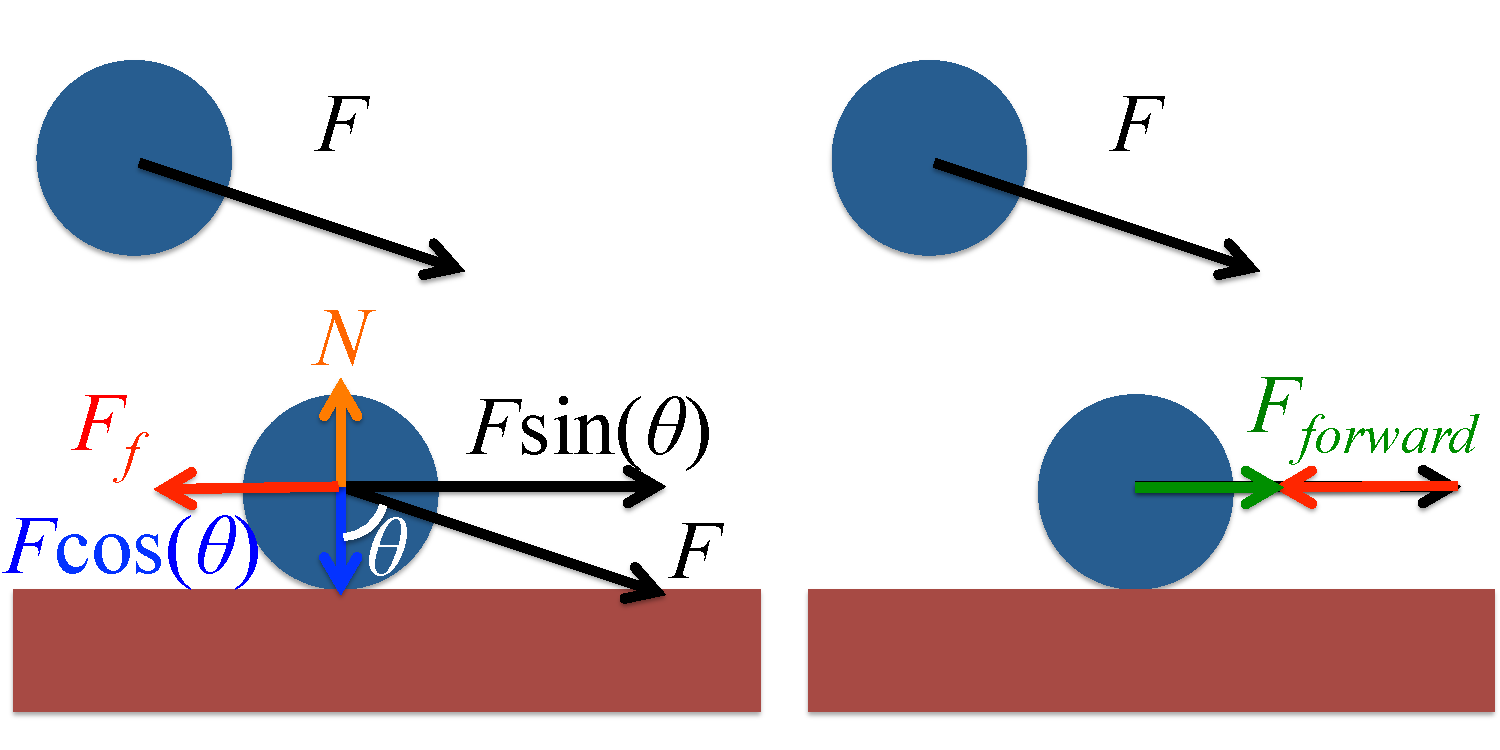
\includegraphics[width=\columnwidth]{friction.pdf} 
\caption{Wall friction reduces the force for going forward $F_{\text{\emph{forward}}}$ on a robot near a wall, but not for a free robot.}
\label{fig:friction}
\end{center}
\end{figure} 




\subsection{Position control of $2$ robots using wall friction}\label{sec:PostionControl2Robots}
\begin{figure*}
\centering
\renewcommand{\figwid}{0.4\columnwidth}
{\begin{overpic}[width =\figwid]{one_1.jpg}\put(45,75){$t$ = 0 s}
\end{overpic}
\begin{overpic}[width =\figwid]{one_2.jpg}\put(45,75){$t$ = 0.25 s}
\end{overpic}
\begin{overpic}[width =\figwid]{one_3.jpg}\put(45,75){$t$  = 0.5 s}
\end{overpic}
\begin{overpic}[width =\figwid]{one_4.jpg}\put(45,75){$t$  = 0.75 s}
\end{overpic}
\begin{overpic}[width =\figwid]{one_5.jpg}\put(45,75){$t$  = 1 s}
\end{overpic}}\\
%{\begin{overpic}[width =\figwid]{two_1.jpg}\put(45,75){$t$  = 0 s}
%\end{overpic}
%\begin{overpic}[width =\figwid]{two_2.jpg}\put(45,75){$t$  = 0.25 s}
%\end{overpic}
%\begin{overpic}[width =\figwid]{two_3.jpg}\put(45,75){$t$  = 0.5 s}
%\end{overpic}
%\begin{overpic}[width =\figwid]{two_4.jpg}\put(45,75){$t$  = 0.75 s}
%\end{overpic}
%\begin{overpic}[width =\figwid]{two_5.jpg}\put(45,75){$t$  = 1 s}
%\end{overpic}}\\
\vspace{.5em}
{\begin{overpic}[width =\figwid]{S3_1.jpg}\put(45,75){$t$ = 0 s}
\end{overpic}
\begin{overpic}[width =\figwid]{S3_2.jpg}\put(45,75){$t$ = 0.25 s}
\end{overpic}
\begin{overpic}[width =\figwid]{S3_3.jpg}\put(45,75){$t$  = 0.5 s}
\end{overpic}
\begin{overpic}[width =\figwid]{S3_4.jpg}\put(45,75){$t$  = 0.75 s}
\end{overpic}
\begin{overpic}[width =\figwid]{S3_5.jpg}\put(45,75){$t$  = 1 s}
\end{overpic}}
\vspace{-1em}

\caption{\label{fig:shapeControlMathematica1}{Frames from an implementation of Alg.\ \ref{alg:PosControl2Robots}: two robot positioning using walls with infinite friction. The algorithm only requires friction along the bottom and left walls.
Robot initial positions are shown by a crosshair, and final positions by a circled crosshair.  Dashed lines show the shortest route if robots could be controlled independently.  The path given by  Alg.\ \ref{alg:PosControl2Robots} is shown with solid arrows.
The bottom row shows an extreme case where the robots must switch position.
}
%\vspace{-2em}
}
\end{figure*}

This section describes Alg.~\ref{alg:PosControl2Robots}, an algorithm that uses wall-friction to arbitrarily position two robots in a rectangular workspace.  This algorithm  introduces concepts that will be used for multi-robot positioning. It only requires collisions with two orthogonal walls, in this case, the bottom and left walls. Fig.~\label{fig:shapeControlMathematica1} shows a Mathematica implementation of the algorithm, and is useful as a visual reference for the following description.

Assume two robots are initialized at $s_1$ and $s_2$ with corresponding goal destinations $e_1$ and $e_2$. 
Denote the current positions of the robots  $r_1$ and $r_2$. 
Subscripts $_x$ and $_y$ denote the $x$ and $y$ coordinates, i.e., $s_{1x}$ and $s_{1y}$ denote the $x$ and $y$ locations of $s_1$. 
The algorithm assigns a global control input at every instance.
 As a result, our goal is to adjust 
 $\Delta r_x = r_{2x}-r_{1x}$ from $\Delta s_x = s_{2x}-s_{1x}$ to $\Delta e_x = e_{2x}-e_{1x}$ and  adjust 
 $\Delta r_y = r_{2y}-r_{1y}$ from $\Delta s_y = s_{2y}-s_{1y}$ to $\Delta e_y = e_{2y}-e_{1y}$ using a shared global control input. 
 This algorithm exploits the position-dependent friction model \eqref{eq:frictionmodel}.
 %employing the assumption we have made earlier about the walls' friction. 

Our algorithm solves the positioning problem in two steps: 
First, $|\Delta r_x - \Delta e_x |$ is reduced to zero while  $\Delta r_y$ is kept constant in Alg.~\ref{alg:XControl}. 
Second $|\Delta r_y - \Delta e_y |$ is reduced to zero while  $\Delta r_x$ is kept constant in Alg.~\ref{alg:YControl}. 

Step (i): Fixing $\Delta r_x$
\label{theory:step1}
\begin{enumerate}
\item Define $ \Delta s_x  = s_{1x} - s_{2x} $ and $ \Delta e_x = e_{1x} - e_{2x}$.
If $\Delta e_x$ is negative, the robots will be commanded to move toward the left wall and halt $\epsilon$ distance from the left wall.
If $\Delta e_x \ge 0$, the robots will be commanded to move toward the right wall and halt $\epsilon$ distance from the right wall. The epsilon distance prevents the robots from experiencing friction along the vertical wall.
\item  let $y_{\min} = \min_i r_{iy}$, i.e., $y_{\min}$ be the minimum height of the two robots. Move both robots downward  $y_{\min}$ such that one of the robots touches the bottom wall and hence friction force will prevent this robot from moving left or right.
\item friction force holds the lower robot in place while the upper robot may move right and left freely to change $\Delta r_x $ to $\Delta e_x$.
\item  If after the free move of the upper robot $\Delta r_x$ is not $\Delta e_x$, Step (i) will be repeated.  No more than two iterations of step (i) are required.
\end{enumerate}

Step (ii): Fixing $\Delta r_y$
Now that $\Delta r_x$ is corrected, $\Delta r_y$ must be corrected:
\begin{enumerate}
\item Define  $ \Delta s_y  = s_{1y} - s_{2y} $ and  $ \Delta e_y = e_{1y} - e_{2y}.$
If $\Delta e_y$ is negative, the robots will be commanded to move toward the top wall and halt $\epsilon$ distance from the top wall.
If $\Delta e_y \ge 0$, the robots will be commanded to move toward the bottom wall and halt $\epsilon$ distance from the bottom wall. The epsilon distance prevents the robots from experiencing friction along the horizontal wall.
\item  let $x_{\min} = \min_i r_{ix}$, i.e., $x_{\min}$ be the minimum distance of the two robots from the origin along the $x$-axis. Move both robots to the left $x_{\min}$ such that one of the robots  touches the left wall and hence friction force will prevent this robot from moving up or down.
\item  friction force holds the left robot in place while the right robot may move up or down freely to change $\Delta r_y $  to $\Delta e_y$.
\item  If after the free move of the right robot $\Delta r_y$ is not $\Delta e_y$, Step (ii) will be repeated.  No more than two iterations of step (ii) are required.
\end{enumerate}
Once $\Delta r_x$ and $\Delta r_y$ are set to $\Delta e_x$ and $\Delta e_y$, we can use global input to easily move both robots from $r_1$ and $r_2$ toward $e_1$ and $e_2$. 


\begin{algorithm}
\caption{WallFrictionArrange2Robots($s_1,s_2,e_1,e_2,L$)}\label{alg:PosControl2Robots}
\begin{algorithmic}[1]
\Require 
Knowledge of starting $(s_1,s_2)$ and ending $(e_1,e_2)$ positions of  two robots. 
$(0,0)$ is bottom corner, $s_1$ is rightmost robot, 
 $L$ is length of the walls. 
 Current position of the robots are $(r_1,r_2)$.

\State ($r_1,r_2$) = GenerateDesired$x$-spacing($s_1,s_2,e_1,e_2,L$)
\State GenerateDesired$y$-spacing($r_1,r_2,e_1,e_2,L$)

\end{algorithmic}
\end{algorithm}


\begin{algorithm}
\caption{GenerateDesired$x$-spacing($s_1,s_2,e_1,e_2,L$)}\label{alg:XControl}
\begin{algorithmic}[1]
\Require Knowledge of starting $(s_1,s_2)$ and ending $(e_1,e_2)$ positions of  two robots. 
$(0,0)$ is bottom corner, $s_1$ is topmost robot, 
 $L$ is length of the walls. Current robot positions are $(r_1,r_2)$.
\Ensure   $ r_{1y} - r_{2y}  \equiv s_{1y} - s_{2y} $   %$\Delta y(t) \equiv \Delta y(0)$ 
\State $\epsilon \gets $ small number
\State $ \Delta s_x  \gets s_{1x} - s_{2x} $
\State $ \Delta e_x \gets e_{1x} - e_{2x} $
\State $ r_1 \gets s_1$, $ r_2 \gets s_2$
\If {$\Delta e_x < 0 $ }
\State $ m \gets ( L-\epsilon-\max( r_{1x},r_{2x}) ,0)   $ \Comment{Move to right wall}
\Else 
\State  $ m \gets ( \epsilon-\min( r_{1x},r_{2x}),0 )    $ \Comment{Move to left wall}
\EndIf
\State $m  \gets  m + (0, -\min( r_{1y},r_{2y} ))$ \Comment{Move to bottom}
\State $ r_1 \gets r_1+m$, $ r_2 \gets r_2+m$ \Comment{Apply move}
\If {$\Delta e_x - (r_{1x} - r_{2x} ) > 0 $}
\State $ m \gets (\min(|\Delta e_x - \Delta s_x |, L- r_{1x}), 0)$  \Comment{Move right}
\Else
\State $ m \gets (-\min(|\Delta e_x - \Delta s_x |, r_{1x}), 0)$\Comment{Move left}
\EndIf 
\State $m  \gets  m + (0, \epsilon)$ \Comment{Move up}
\State $ r_1 \gets r_1+m$, $ r_2 \gets r_2+m$ \Comment{Apply move}
\State $\Delta r_x = r_{1x} - r_{2x}$
\If {$\Delta r_x \equiv \Delta e_x$} 
%\State   $ m \gets (e_{1x}-r_{1x}, e_{1y}-r_{1y})$
%\State $ r_1 \gets r_1+m$, $ r_2 \gets r_2+m$ \Comment{Apply move}
\State  \Return $(r_1,r_2)$
\Else   
\State \Return GenerateDesired$x$-spacing($r_1,r_2,e_1,e_2,L$)
\EndIf
\end{algorithmic}
\end{algorithm}

\begin{algorithm}
\caption{GenerateDesired$y$-spacing($s_1,s_2,e_1,e_2,L$)}\label{alg:YControl}
\begin{algorithmic}[1]
\Require Knowledge of starting $(s_1,s_2)$ and ending $(e_1,e_2)$ positions of  two robots. 
$(0,0)$ is bottom corner, $s_1$ is rightmost robot, 
 $L$ is length of the walls. Current position of the robots are $(r_1,r_2)$.
\Ensure   $ r_{1x} - r_{2x}  \equiv s_{1x} - s_{2x} $   %$\Delta y(t) \equiv \Delta y(0)$ 
\State $ \Delta s_y  \gets s_{1y} - s_{2y} $
\State $ \Delta e_y \gets e_{1y} - e_{2y} $
\State $ r_1 \gets s_1$, $ r_2 \gets s_2$
\If {$\Delta e_y < 0 $ }
\State $ m \gets ( L-\max( r_{1y},r_{2y}) ,0)   $ \Comment{Move to top wall}
\Else 
\State  $ m \gets ( -\min( r_{1y},r_{2y}),0 )    $ \Comment{Move to bottom wall}
\EndIf
\State $m  \gets  m + (0, -\min( r_{1x},r_{2x} ))$ \Comment{Move to left}
\State $ r_1 \gets r_1+m$, $ r_2 \gets r_2+m$ \Comment{Apply move}
\If {$\Delta e_y - (r_{1y} - r_{2y} ) > 0 $}
\State $ m \gets (\min(|\Delta e_y - \Delta s_y |, L- r_{1y}), 0)$  \Comment{Move top}
\Else
\State $ m \gets (-\min(|\Delta e_y - \Delta s_y |, r_{1y}), 0)$\Comment{Move bottom}
\EndIf 
\State $m  \gets  m + (0, \epsilon)$ \Comment{Move right}
\State $ r_1 \gets r_1+m$, $ r_2 \gets r_2+m$ \Comment{Apply move}
\State $\Delta r_y = r_{1y} - r_{2y}$
\If {$\Delta r_y \equiv \Delta e_y$} 
\State   $ m \gets (e_{1x}-r_{1x}, e_{1y}-r_{1y})$
\State $ r_1 \gets r_1+m$, $ r_2 \gets r_2+m$ \Comment{Apply move}
\State  \Return $(r_1,r_2)$
\Else   
\State \Return GenerateDesired$y$-spacing($r_1,r_2,e_1,e_2,L$)
\EndIf
\end{algorithmic}
\end{algorithm}






\subsection{Position Control of $n$ robots using wall friction}\label{sec:PostionControlnRobots}
Algorithm \ref{alg:PosControl2Robots}  can be extended to control the position of $n$ robots using wall friction under several constraints. The solution described here is an iterative procedure with $n$ loops. The $k$th loop moves the $k$th robot from a \emph{staging zone} to the desired position in a \emph{build zone}. At the end the $k$th loop, robots 1 through $k$ are in their desired final configuration in the build zone, and robots $k+1$ to $n$ are in the staging zone. See Fig.~\ref{fig:construction2d} for a schematic of the build and staging zones.



\begin{figure}
\begin{center}
	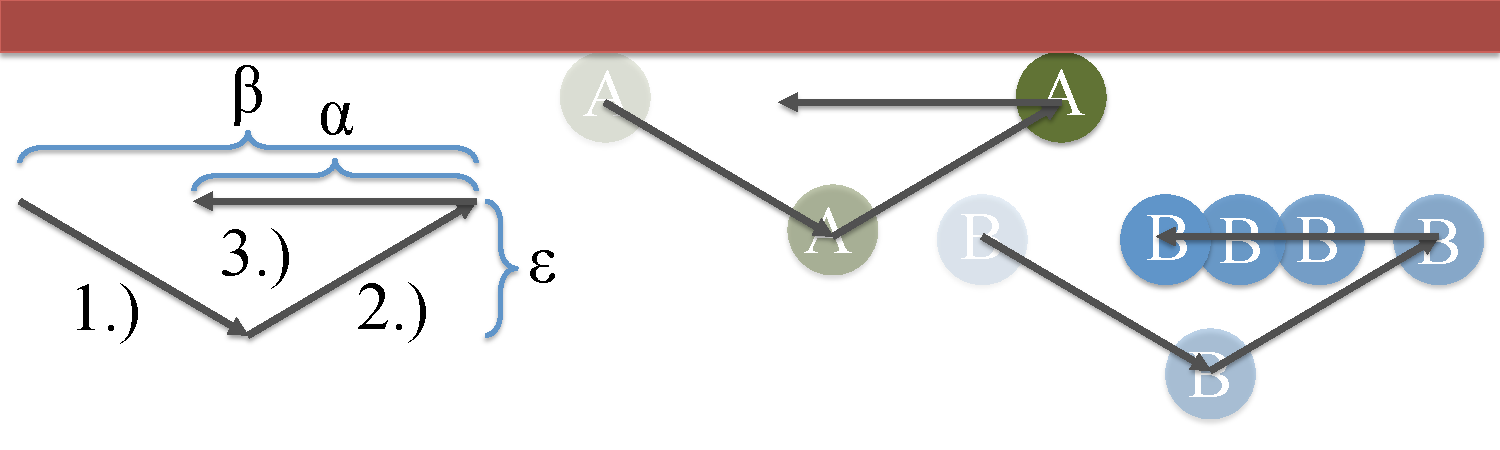
\includegraphics[width=1.0\columnwidth]{driftmove.pdf}
\end{center}
\caption{\label{fig:driftmove}
A  $\operatorname{DriftMove}(\alpha, \beta, \epsilon)$ to the right consists of repeating a triangular movement sequence $\{ (\beta/2,-\epsilon),(\beta/2,\epsilon),(-\alpha,0)\}$. The robot $A$ touching a top wall will move right $\beta$ units, while robots not touching the top move right $\beta-\alpha$.
}
\end{figure}
\begin{figure}
\begin{center}
	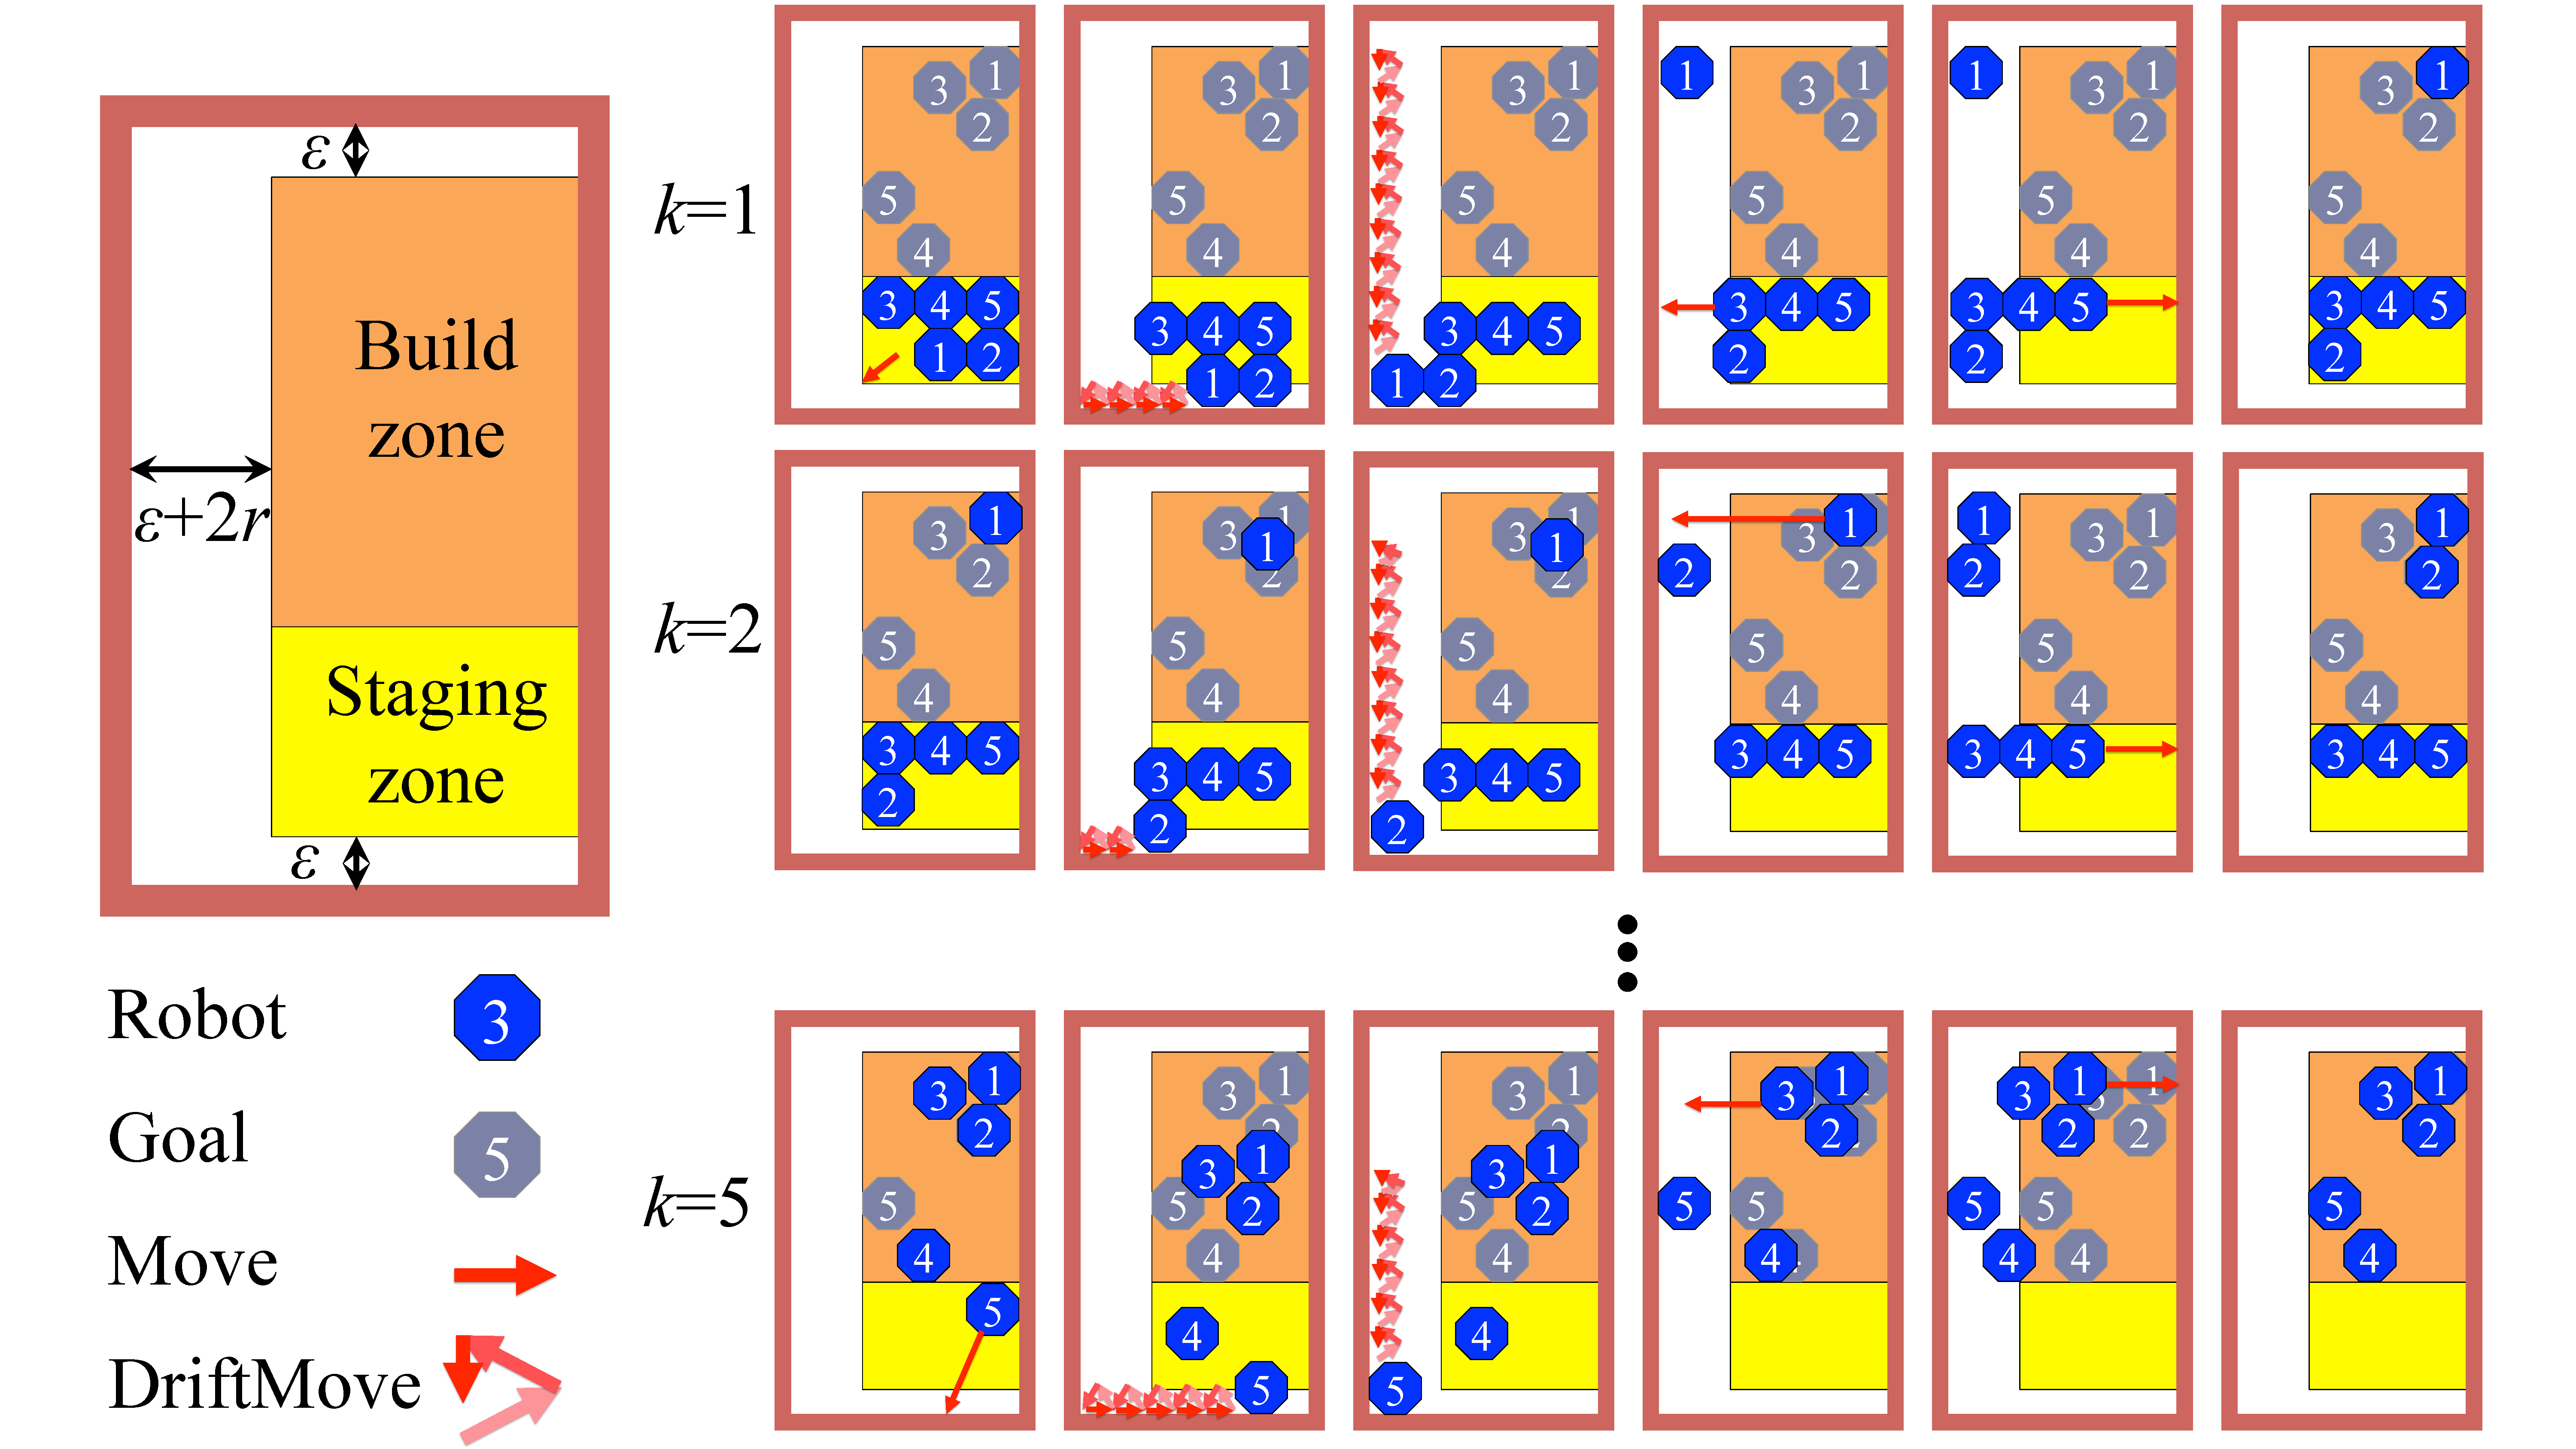
\includegraphics[width=1.0\columnwidth]{PositionNrobots.pdf}
\end{center}
\caption{\label{fig:construction2d}
Illustration of Alg.\ \ref{alg:PosControlNRobots}, $n$ robot position control  using wall friction.
}
\end{figure}


Assume an open workspace with four axis-aligned walls with infinite friction.
The axis-aligned build zone of dimension $(w_b, h_b)$ containing the final configuration of $n$ robots must be disjoint from the axis-aligned staging zone of dimension $(w_s, h_s)$  containing the starting configuration of $n$ robots. Without loss of generality, assume the build zone  is above the staging zone. 
Furthermore, there must be at least $\epsilon$ space above the build zone, $\epsilon$ below the staging zone, and $\epsilon + 2r$ to the left of the build and staging zone, where $r$ is the radius of a robot.  The minimum workspace is then $(\epsilon + 2r + \max(w_f,w_s), 2\epsilon + h_s,h_f)$.

The $n$ robot position control algorithm relies on a $\operatorname{DriftMove}(\alpha, \beta, \epsilon)$ control input, shown in Fig.\  \ref{fig:driftmove}.
A drift move consists of repeating a triangular movement sequence $\{ (\beta/2,-\epsilon),(\beta/2,\epsilon),(-\alpha,0)\}$. The robot touching a top wall moves right $\beta$ units, while robots not touching the top move right $\beta-\alpha$.

Let $(0,0)$ be the lower left corner of the workspace, $p_k$ the $x,y$ position of the $k$th robot, and $f_k$ the final $x,y$ position of the $k$th robot. Label the robots in the staging zone from left-to-right and top-to-bottom, and the $f_k$ configurations right-to-left and top-to-bottom as shown in Fig.~\ref{fig:construction2d}.

\begin{algorithm}
\caption{PositionControl$n$RobotsUsingWallFriction($k$)}\label{alg:PosControlNRobots}
\begin{algorithmic}[1]
\State move( $-\epsilon, r-p_{k,y}$) % move  away from right wall and down till robot k touches bottom


\While{ $p_{k,x} > r$} 
\State $\operatorname{DriftMove}(\epsilon, \min(p_{k,x} - r,\epsilon), \epsilon)$ left   %drift move left until kth robot touches left wall
\EndWhile

\State $m \gets \operatorname{ceil}(\frac{f_{k,y}-r}{\epsilon})$
\State $\beta \gets \frac{f_{k,y}-r}{m}$
\State $\alpha \gets \beta - \frac{r - p_{k,y}-\epsilon}{m}$
\For{ $m$ iterations}
\State $\operatorname{DriftMove}(\alpha, \beta, \epsilon)$ up   %move kth robot to f_{ky} and leave the rest in position.
\EndFor

\State move($r+\epsilon-f_{k,x}, 0$)  % move the group to the left until k is in the correct relative x position
\State move($f_{k,x}-r, 0$)  

\end{algorithmic}
\end{algorithm}

Alg. \ref{alg:PosControlNRobots} procedes as follows:  
First, the robots are moved left away from right wall, and down so robot $k$ touches the bottom wall.
Second, a set of $\operatorname{DriftMove()}$s are executed that move robot $k$ to the left wall with no net movement of the other robots.
Third, a set of $\operatorname{DriftMove()}$s are executed that  move robot $k$ to its target height and return the other robots to their initial heights. 
Fourth, all robots except robot $k$ are pushed left until robot $k$ is in the correct relative $x$ position compared to robots 1 to $k-1$.

Finally, all robots are moved right until robot $k$ is in the desired target position.


\subsection{Controlling Covariance Using Wall Friction}
We can use friction to control covariance of the swarm. 

\begin{algorithm}
\caption{Swarm Covariance Control With Wall Friction}\label{alg:CovCont}
\begin{algorithmic}[1]
\Require Swarm is Gaussian Distributed(in limit it is uniformly distributed)
\Require L is the length of the $x$ of the workspace
\While $\bar{x}< L - \sigma_x(t)$
\State Go Left
\EndWhile
\State Go Up for ...
\end{algorithmic}
\end{algorithm}







